\documentclass[12pt,a4paper,oneside]{article}

\usepackage[T1]{fontenc}
\usepackage[utf8]{inputenc}
\usepackage[english]{babel}

\usepackage{amssymb}
\usepackage{amsmath}
\usepackage{amsthm}
\usepackage{graphicx}
\usepackage{tikz}
\usepackage{setspace}
\usepackage{url}
\usepackage{booktabs}
\usepackage{array}
\usepackage{longtable}
\usepackage{tabularx}
\usepackage{float}
\usepackage{enumitem}
\usepackage[round,authoryear]{natbib}
\usepackage[colorlinks=true, linkcolor=black, citecolor=black, urlcolor=black]{hyperref}
\usepackage{geometry}
\usepackage{caption}
\usepackage{xcolor}
\usepackage{listings}
\usepackage{courier}
\usepackage{tocloft}
\usepackage{multirow}
\usepackage{pdflscape}
\usepackage{adjustbox}

\usetikzlibrary{arrows.meta, positioning, shapes.geometric, calc}

\geometry{margin=2.5cm}
\setstretch{1.15}

\renewcommand{\cftsecleader}{\hfill}
\renewcommand{\cftsubsecleader}{\hfill}

\lstdefinestyle{solidity}{
    basicstyle=\footnotesize\ttfamily,
    breaklines=true,
    frame=single,
    columns=fullflexible,
    keepspaces=true,
    showstringspaces=false,
    keywordstyle=\bfseries,
    commentstyle=\itshape,
    tabsize=2
}

\theoremstyle{definition}
\newtheorem{defi}{Definition}
\newtheorem{satz}{Theorem}
\theoremstyle{plain}

\begin{document}

\thispagestyle{empty}
\begin{titlepage}
    \begin{center}
        \begin{minipage}{0.3\linewidth}
            \IfFileExists{HTW_Logo.jpg}
                {\includegraphics[height=3cm]{HTW_Logo}}
                {\IfFileExists{HTW_Logo.pdf}
                    {\includegraphics[height=3cm]{HTW_Logo}}
                    {\fbox{\parbox[c][3cm][c]{4cm}{\centering HTW Logo}}}}
        \end{minipage}
        \begin{minipage}{0.6\linewidth}
            \textsf{
                \begin{flushright}
                    Department of Computer Science,\\ Communication and Economics \\
                    HTW Berlin
                \end{flushright}
            }
        \end{minipage}\\[90pt]

        \begin{doublespace}
            {\Huge\textbf{AI Agents and the Need for Crypto-Payment}}\\[40pt]
        \end{doublespace}

        {\Large Seminar Paper \\[6pt] Blockchain Business Development }\\[40pt]

        by\\
        {\scshape\large Andrea Rivadossi \\
        Matteo Capoferri\\
        Igor Hebda\\
        Panth Patel}\\[30pt]

        submitted to \\[6pt]

        {\large Prof. Dr.-Ing. Katarina Krüger} \\[30pt]

        {Berlin, \today}
    \end{center}
\end{titlepage}

\tableofcontents
\newpage
\section{Introduction}

The growing operational autonomy of AI agents creates tension with traditional financial infrastructure. Banking systems, card networks, and conventional payment infrastructure were designed primarily for human users and organizational account holders. Traditional payment systems rely on explicit authorization, relatively infrequent transactions, and payment values large enough to absorb compliance, processing, and administrative costs. AI agents fit this model poorly because their behavior is automated, repetitive, time-sensitive, and often based on extremely small units of value \citep{mougayar2016}. A machine may need to purchase thousands of small resource units continuously and in real time, fundamentally changing the logic of payment execution. Payment therefore becomes embedded directly into the technical workflow rather than remaining a separate commercial activity \citep{krueger2026workshop2,krueger2026workshop3}.

The objective of this report is to evaluate whether blockchain-based programmable settlement can reduce operational limitations present in existing payment systems in selected machine-to-machine payment scenarios. The analysis focuses on the conditions under which blockchain-based payment infrastructure becomes economically and technically justified. The analytical framework combines stakeholder analysis, decision-path analysis, use-value analysis, and blockchain modeling \citep{krueger2026workshop1,krueger2026workshop3,krueger2026workshop5,krueger2026workshop7a,krueger2026workshop7b}. In addition, the analysis includes a process model based on BPMN logic, a minimal smart contract prototype, and a supervisory dashboard mock-up illustrating how bounded automation could operate in practice.

Several blockchain-related AI use cases are identified and evaluated. These include autonomous purchase of real-time data, decentralized compute rental, access to DePIN infrastructure, and use of modular digital services. Autonomous purchase of real-time data and narrowly scoped digital resources is selected as the primary use case and translated into a blockchain model involving AI agents, resource providers, smart contracts, stable digital assets, oracles, and human supervisors. Particular attention is given to governance mechanisms, bounded autonomy, operational security, incentive alignment, and accountability structures required for delegating payment authority to software systems. The proposed architecture is also placed within the broader European regulatory environment shaped by MiCA and the AI Act \citep{europeanparliament2023mica,europeanunion2024aiact}. 

\section{Use Case Identification and Selection}

Several candidate blockchain use cases for autonomous AI agents are considered in the analysis. At this stage, the goal is not detailed modeling, but identification of scenarios in which programmable blockchain-based settlement could create operational or economic value \citep{krueger2026workshop5}.

The candidate use cases are linked to concrete services, products, processes, and value objects:

\begin{itemize}[leftmargin=1.2cm]
\item \textbf{Real-time data purchase:} weather data, traffic feeds, market signals, industrial sensor data; process: request, verify delivery, trigger payment; value object: narrow machine-readable data unit.
\item \textbf{Compute or storage rental:} short compute bursts, storage blocks, edge compute slots; process: request capacity, verify usage, release payment; value object: temporary infrastructure access.
\item \textbf{DePIN access:} sensor query, device activation, physical resource access; process: request access, verify off-chain action, settle payment; value object: digitally addressable physical service.
\item \textbf{Modular digital services:} micro-APIs, classification services, translation modules, specialized agents; process: API call, result delivery, settle payment; value object: service execution.
\end{itemize}

Table \ref{tab:products_processes_values} summarizes the products or services, processes, and value objects.

\begin{table}[H]
\centering
\caption{Products, processes, and value objects}
\label{tab:products_processes_values}
\begin{tabular}{p{4.2cm}p{4.3cm}p{5.1cm}}
\toprule
\textbf{Product / Service} & \textbf{Process} & \textbf{Value Object} \\
\midrule
Real-time data purchase & Request, verify delivery, settle payment & Machine-readable data unit \\
Compute or storage rental & Request capacity, verify usage, release payment & Temporary infrastructure access \\
DePIN resource access & Request access, verify physical execution, settle payment & Digitally addressable physical service \\
Modular digital service & API call, result delivery, settle payment & Service execution \\
\bottomrule
\end{tabular}
\end{table}

The first screening step is the decision path. For AI agents purchasing low-value resources across multiple providers, the decision path leads to a positive result. The process requires shared transaction state, involves several actors, operates in a partially low-trust environment, and depends on automatic conditional execution. The issue is therefore not just data storage, but coordinated and programmable settlement \citep{krueger2026workshop3}.

\begin{figure}[H]
\centering
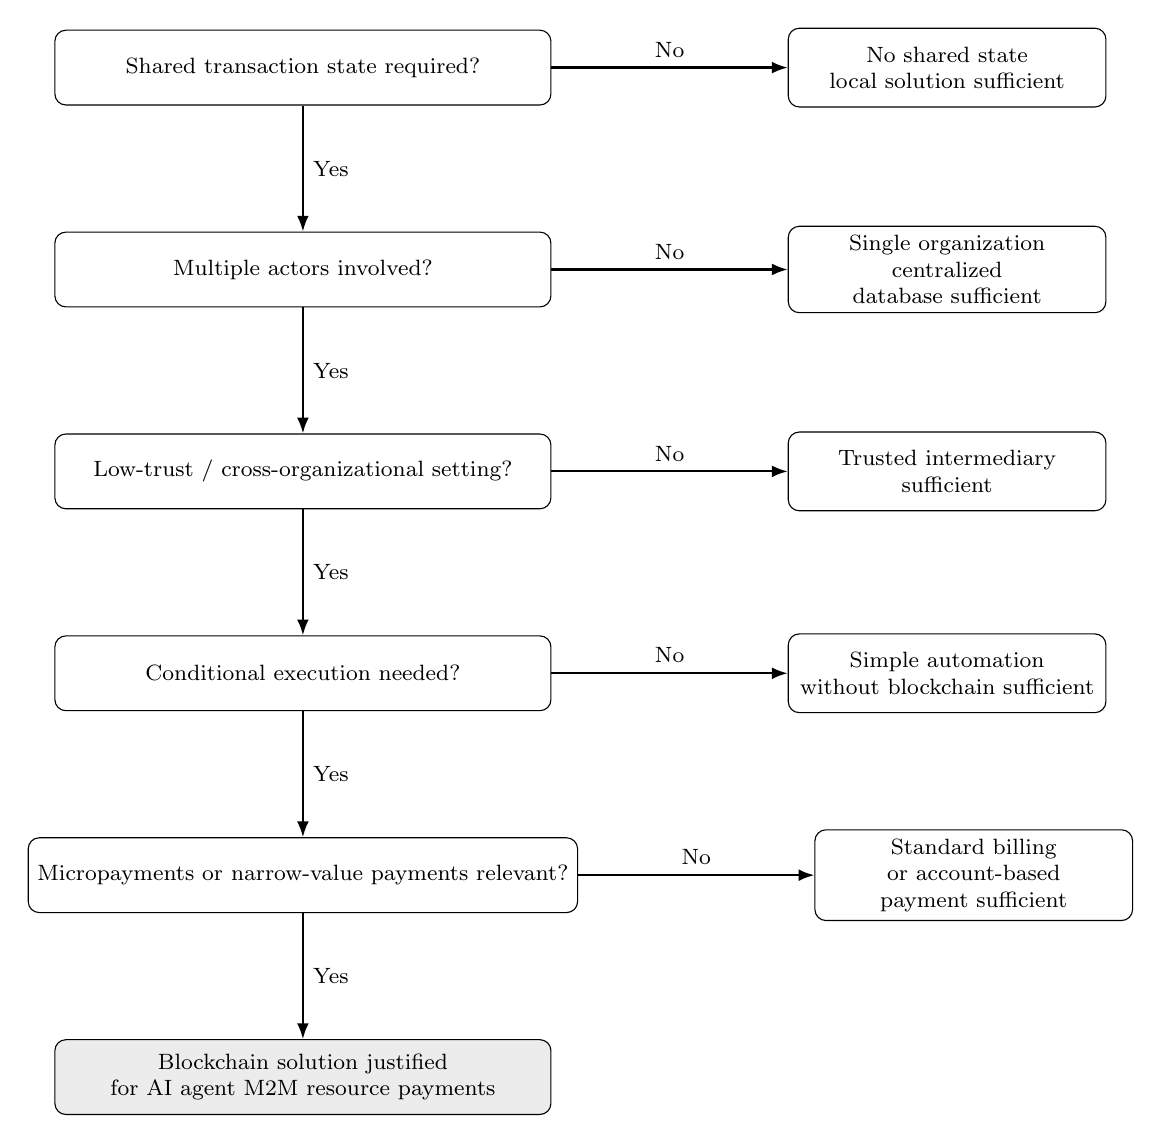
\begin{tikzpicture}[
    node distance=1.6cm,
    every node/.style={font=\footnotesize},
    q/.style={rectangle, rounded corners, draw, align=center, minimum width=6.3cm, minimum height=0.95cm},
    arr/.style={-{Latex[length=2mm]}, thick}
]

\node[q] (q1) {Shared transaction state required?};
\node[q, below=of q1] (q2) {Multiple actors involved?};
\node[q, below=of q2] (q3) {Low-trust / cross-organizational setting?};
\node[q, below=of q3] (q4) {Conditional execution needed?};
\node[q, below=of q4] (q5) {Micropayments or narrow-value payments relevant?};

\node[q, below=of q5, fill=gray!15] (res)
{Blockchain solution justified\\for AI agent M2M resource payments};

\node[
    right=3cm of q1,
    draw,
    rounded corners,
    align=center,
    text width=3.8cm,
    minimum height=1.0cm
] (no0) {No shared state\\local solution sufficient};

\node[
    right=3cm of q2,
    draw,
    rounded corners,
    align=center,
    text width=3.8cm,
    minimum height=1.0cm
] (no1) {Single organization\\centralized database sufficient};

\node[
    right=3cm of q3,
    draw,
    rounded corners,
    align=center,
    text width=3.8cm,
    minimum height=1.0cm
] (no2) {Trusted intermediary\\sufficient};

\node[
    right=3cm of q4,
    draw,
    rounded corners,
    align=center,
    text width=3.8cm,
    minimum height=1.0cm
] (no3) {Simple automation\\without blockchain sufficient};

\node[
    right=3cm of q5,
    draw,
    rounded corners,
    align=center,
    text width=3.8cm,
    minimum height=1.0cm
] (no4) {Standard billing or account-based\\payment sufficient};

\draw[arr] (q1) -- node[right] {Yes} (q2);
\draw[arr] (q2) -- node[right] {Yes} (q3);
\draw[arr] (q3) -- node[right] {Yes} (q4);
\draw[arr] (q4) -- node[right] {Yes} (q5);
\draw[arr] (q5) -- node[right] {Yes} (res);

\draw[arr] (q1.east) -- node[above] {No} (no0.west);
\draw[arr] (q2.east) -- node[above] {No} (no1.west);
\draw[arr] (q3.east) -- node[above] {No} (no2.west);
\draw[arr] (q4.east) -- node[above] {No} (no3.west);
\draw[arr] (q5.east) -- node[above] {No} (no4.west);

\end{tikzpicture}
\caption{Decision path for evaluating blockchain necessity in AI agent payments}
\label{fig:decisionpath}
\end{figure}

The decision path does not prove that blockchain is the best solution. It only shows that the use case passes the initial screening and deserves deeper evaluation. The next step is a more systematic comparison using use-value analysis.


\section{Use-Value Analysis}

After the initial qualitative screening, use-value analysis was applied to compare the candidate use cases in a more systematic way \citep{krueger2026workshop5}. Four candidate processes are evaluated: autonomous purchase of real-time data, decentralized compute rental, access to DePIN-related infrastructure, and procurement of modular digital services by AI agents. Together, these use cases represent the main categories of blockchain-enabled machine-to-machine interaction identified in the earlier analysis.

\subsection{Criteria, Method, and Scoring Scale}

Five criteria were used:

\begin{itemize}[leftmargin=1.2cm]
\item \textbf{Transaction granularity (G):} How strongly does the use case depend on very small or narrowly scoped value units?
\item \textbf{Operational autonomy (A):} To what extent can or should the process be triggered and executed by software with limited human intervention?
\item \textbf{Transparency and auditability (T):} How relevant is verifiable logging and shared state for the process?
\item \textbf{Technical feasibility (F):} How realistic is near-term implementation with existing technology?
\item \textbf{Regulatory controllability (R):} How manageable is the use case from a compliance and governance perspective?
\end{itemize}

Each criterion was evaluated on a four-level scale from 0 to 3. The scale is criterion-specific because each criterion measures a different aspect of suitability.

\begin{table}[H]
\centering
\caption{Criteria, method of investigation, and scoring scale}
\label{tab:scoring_scale}

\begin{adjustbox}{max width=\textwidth}
\begin{tabular}{p{2.6cm}p{2.2cm}p{2.2cm}p{2.2cm}p{2.2cm}p{2.2cm}}
\toprule
\textbf{Criterion} & \textbf{Method} & \textbf{3} & \textbf{2} & \textbf{1} & \textbf{0} \\
\midrule

Transaction granularity (G)
&
Use-case estimation
&
micropayments required
&
small payments useful
&
standard payments sufficient
&
no need for micropayments
\\

Operational autonomy (A)
&
Process analysis
&
fully automatic execution
&
semi-automatic execution
&
frequent human approval needed
&
fully manual process
\\

Transparency and auditability (T)
&
Audit needs assessment
&
public/shared audit trail required
&
internal + external logs important
&
internal logs sufficient
&
no significant audit need
\\

Technical feasibility (F)
&
Technical assessment
&
implementable now with existing tools
&
feasible with moderate integration effort
&
technically complex / limited feasibility
&
currently not realistically feasible
\\

Regulatory controllability (R)
&
Compliance assessment
&
clear bounded controls possible
&
manageable with supervision
&
high compliance uncertainty
&
legally problematic / difficult to justify
\\

\bottomrule
\end{tabular}
\end{adjustbox}
\end{table}

\subsection{Pairwise Comparison and Weighting}

The criteria were weighted by pairwise comparison. In the matrix, a value of 2 means that the column criterion is more important than the row criterion, a value of 1 means that both are equally important, and a value of 0 means that the column criterion is less important than the row criterion. The resulting ranking is \(G > A > T > F = R\).

Transaction granularity and operational autonomy dominate because they express the main mismatch between AI-driven micro-consumption and legacy payment systems. Transparency is important, but secondary. Technical feasibility matters because a concept without practical implementation value is weak. Regulatory controllability is treated as a boundary condition: it is not the main source of utility, but the model is not credible without it.

\begin{table}[H]
\centering
\caption{Pairwise comparison of criteria}
\label{tab:pairwise_explicit}

\begin{tabular}{lccccc}
\toprule
\textbf{Criterion} & \textbf{G} & \textbf{A} & \textbf{T} & \textbf{F} & \textbf{R} \\
\midrule
Transaction granularity (G)       & -- & 0  & 0  & 0  & 1 \\
Operational autonomy (A)          & 2  & -- & 1  & 0  & 0 \\
Transparency and auditability (T) & 2  & 1  & -- & 1  & 0 \\
Technical feasibility (F)         & 2  & 2  & 1  & -- & 1 \\
Regulatory controllability (R)    & 1  & 2  & 2  & 1  & -- \\
\midrule
Total                             & 7  & 5  & 4  & 2  & 2 \\
Interpretation                    & 35\% & 25\% & 20\% & 10\% & 10\% \\
\bottomrule
\end{tabular}
\end{table}


Although technical feasibility and regulatory controllability receive lower weights than transaction granularity, operational autonomy, and auditability, both remain necessary boundary conditions. Technical feasibility determines whether the concept can be implemented with realistic effort, while regulatory controllability determines whether it can be deployed responsibly. For this reason, both criteria are retained in the final weighting at 10\%.


\[
w_G = 0.35,\quad
w_A = 0.25,\quad
w_T = 0.20,\quad
w_F = 0.10,\quad
w_R = 0.10
\]

\subsection{Evaluation of Candidate Processes}

The candidate processes were evaluated qualitatively using the criteria and scoring framework defined above. The qualitative assessments were then translated into numerical values from 0 to 3 for the weighted utility calculation.

\begin{table}[H]
\centering
\caption{Evaluation of candidate processes}
\label{tab:evaluation_criteria}

\begin{adjustbox}{max width=\textwidth}
\begin{tabular}{p{2.8cm}p{2.4cm}p{2.4cm}p{2.6cm}p{2.4cm}}
\toprule

\textbf{Criterion / Process}
&
\textbf{AI purchase of real-time data}
&
\textbf{AI rental of decentralized compute}
&
\textbf{AI access to DePIN sensor/device infrastructure}
&
\textbf{AI procurement of modular digital services}
\\

\midrule

Transaction granularity (G)
&
micropayments required
&
micropayments required
&
micropayments required
&
small payments useful
\\

Operational autonomy (A)
&
fully automatic execution
&
fully automatic execution
&
semi-automatic execution
&
semi-automatic execution
\\

Transparency and auditability (T)
&
internal + external logs important
&
internal + external logs important
&
public/shared audit trail required
&
internal logs sufficient
\\

Technical feasibility (F)
&
implementable now with existing tools
&
feasible with moderate integration effort
&
feasible with moderate integration effort
&
feasible with moderate integration effort
\\

Regulatory controllability (R)
&
manageable with supervision
&
high compliance uncertainty
&
high compliance uncertainty
&
manageable with supervision
\\

\bottomrule
\end{tabular}
\end{adjustbox}
\end{table}

\subsection{Utility Value Calculation}

The weighted utility value was calculated as:

\[
U =
0.35 \cdot G +
0.25 \cdot A +
0.20 \cdot T +
0.10 \cdot F +
0.10 \cdot R
\]

where \(G\) denotes transaction granularity, \(A\) operational autonomy, \(T\) transparency and auditability, \(F\) technical feasibility, and \(R\) regulatory controllability.

\begin{table}[H]
\centering
\caption{Utility value calculation}
\label{tab:utility_value}

\begin{adjustbox}{max width=\textwidth}
\begin{tabular}{p{3.2cm}cccc}
\toprule

\textbf{Criterion}
&
\textbf{AI purchase of real-time data}
&
\textbf{AI rental of decentralized compute}
&
\textbf{AI access to DePIN}
&
\textbf{AI procurement of modular digital services}
\\

\midrule

Transaction granularity (G) & 3 & 3 & 3 & 2 \\
Operational autonomy (A) & 3 & 3 & 2 & 2 \\
Transparency and auditability (T) & 2 & 2 & 3 & 1 \\
Technical feasibility (F) & 3 & 2 & 2 & 2 \\
Regulatory controllability (R) & 2 & 1 & 1 & 2 \\

\midrule

Total result & 13 & 11 & 11 & 9 \\
Weighted result & 2.75 & 2.40 & 2.35 & 1.80 \\
Ranking & 1 & 2 & 3 & 4 \\

\bottomrule
\end{tabular}
\end{adjustbox}
\end{table}

The evaluation identifies autonomous purchase of real-time data as the strongest candidate use case. This scenario combines high transaction granularity, strong operational autonomy, sufficient auditability, high technical feasibility, and manageable regulatory constraints.

Decentralized compute rental achieves the second-highest result. Although the process also benefits from granular machine-to-machine settlement, implementation complexity and regulatory uncertainty are higher. Access to DePIN-related infrastructure performs well in terms of transparency and auditability, but depends more heavily on hardware integration and reliable oracle mechanisms.

Procurement of modular digital services receives the lowest score because many such services can already be supported efficiently through conventional API billing and centralized payment models. As a result, the additional utility created by blockchain-based settlement is comparatively weaker.

Based on the use-value analysis, the remainder of the report focuses on a use case in which an AI agent autonomously purchases real-time data or narrowly scoped digital resource units and settles payments incrementally through blockchain-based digital assets.

\section{Morphological Analysis}

To complement the use-value analysis, the selected use case was additionally examined using a morphological box. The purpose of this step is not to replace the ranking logic, but to identify alternative design configurations and evaluate which combinations of features best support the proposed blockchain-based settlement model. This is relevant because the same operational use case may be implemented through different governance structures, settlement mechanisms, and infrastructure architectures.


\begin{table}[H]
\centering
\caption{Morphological box for the AI-agent micropayment use case}
\label{tab:morphological}
\begin{tabular}{p{3.4cm}p{3.0cm}p{3.0cm}p{3.0cm}}
\toprule
\textbf{Feature} & \textbf{Option 1} & \textbf{Option 2} & \textbf{Option 3} \\
\midrule
Payment unit & Fixed micropayment & Dynamic usage-based price & Subscription bundle \\
Oracle structure & Centralized oracle & Decentralized oracle & Consensus-based oracle set \\
Blockchain type & Public permissionless & Hybrid / semi-public & Private permissioned \\
Settlement asset & Stablecoin & Native network token & Fiat-backed tokenized claim \\
Provider access & Approved whitelist & Reputation-based access & Open marketplace \\
Automation level & Fully automatic & Semi-automatic with thresholds & Manual release \\
Approval logic & Single supervisor & Multi-signature governance & Escalation workflow \\
Data storage & Mostly off-chain & Mixed on-/off-chain & Extended on-chain proofs \\
\bottomrule
\end{tabular}
\end{table}

The preferred configuration combines a hybrid or public smart-contract environment with stablecoin-based settlement, approved providers, predominantly off-chain service data, and automatic execution below predefined thresholds. This configuration reflects the broader principle of bounded autonomy applied throughout the report. It also allows governance and oracle structures to become progressively stricter in scenarios involving higher-value transactions or increased operational risk.

\section{Stakeholders, Business Logic, and Added Value}

The selected use case involves several stakeholder groups, including AI owners or deploying organizations, AI developers, resource providers, blockchain infrastructure operators, stablecoin issuers, regulators, auditors, and end users affected by AI-enabled services. These actors differ in their operational influence, economic interests, and ability to support or constrain adoption, which makes stakeholder mapping necessary \citep{krueger2026workshop1}.

AI owners are the primary adoption actors because they carry the operational and financial risks associated with delegating payment authority to software systems. Regulators remain influential because they define the legal boundaries within which autonomous payment processes may operate. Resource providers are essential because the proposed architecture depends on their willingness to expose data or service units in machine-readable and billable form. Auditors and security specialists also play an important role because trust in the system depends on verifiable contract logic, governance mechanisms, and operational controls.


\begin{figure}[H]
\centering
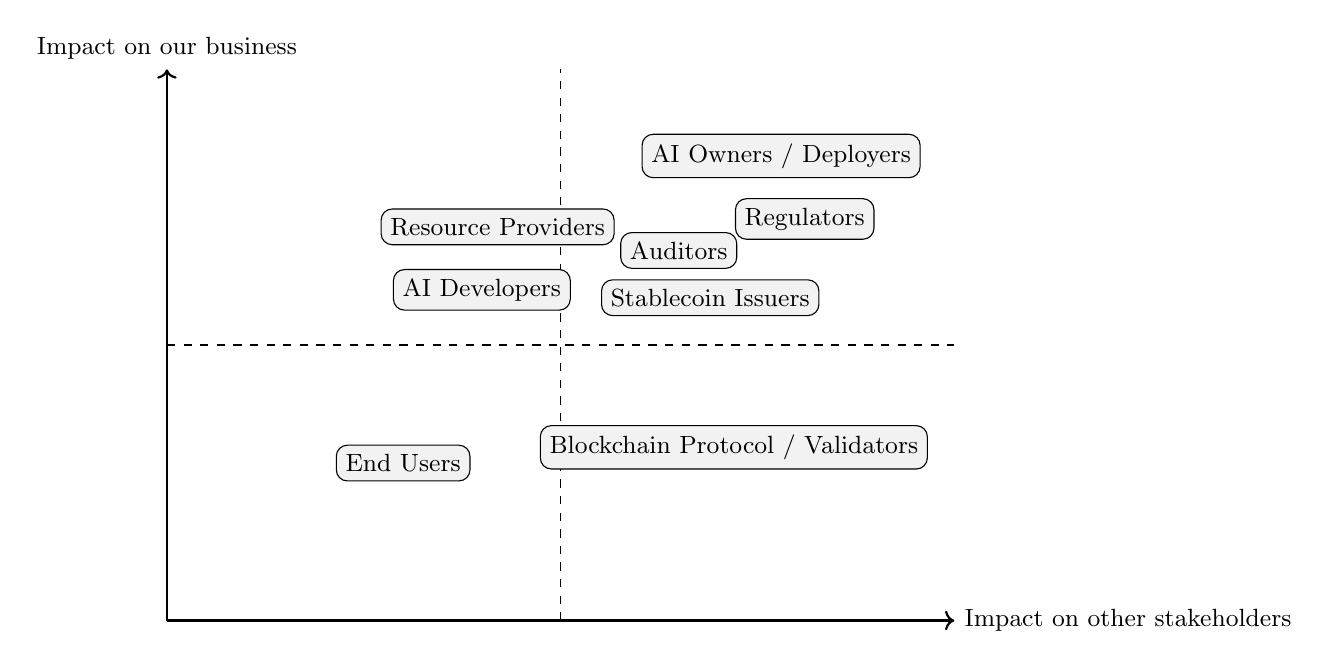
\begin{tikzpicture}[scale=1.0, every node/.style={font=\small}]
    \draw[->, thick] (0,0) -- (10,0) node[right] {Impact on other stakeholders};
    \draw[->, thick] (0,0) -- (0,7) node[above] {Impact on our business};

    \draw[dashed] (5,0) -- (5,7);
    \draw[dashed] (0,3.5) -- (10,3.5);

    \node[draw, rounded corners, fill=gray!10] at (7.8,5.9) {AI Owners / Deployers};
    \node[draw, rounded corners, fill=gray!10] at (8.1,5.1) {Regulators};
    \node[draw, rounded corners, fill=gray!10] at (6.5,4.7) {Auditors};
    \node[draw, rounded corners, fill=gray!10] at (6.9,4.1) {Stablecoin Issuers};
    \node[draw, rounded corners, fill=gray!10] at (4.2,5.0) {Resource Providers};
    \node[draw, rounded corners, fill=gray!10] at (4.0,4.2) {AI Developers};
    \node[draw, rounded corners, fill=gray!10] at (7.2,2.2) {Blockchain Protocol / Validators};
    \node[draw, rounded corners, fill=gray!10] at (3.0,2.0) {End Users};
\end{tikzpicture}
\caption{Stakeholder map based on impact on business and other stakeholders}
\label{fig:stakeholdermap}
\end{figure}

To complement the stakeholder map, the analysis includes a structured stakeholder matrix.

\begin{landscape}

\footnotesize
\setlength{\extrarowheight}{2pt}
\setlength{\tabcolsep}{4pt}

\begin{longtable}{p{3.0cm}p{3.2cm}p{1.2cm}p{1.3cm}p{3.6cm}p{3.6cm}p{3.6cm}p{3.8cm}}
\caption{Stakeholder analysis matrix}
\label{tab:stakeholdermatrix}\\
\toprule
\textbf{Stakeholder} &
\textbf{Contact / Role} &
\textbf{Impact} &
\textbf{Influence} &
\textbf{What is important?} &
\textbf{How can they support the project?} &
\textbf{How can they block the project?} &
\textbf{Engagement strategy} \\
\midrule
\endfirsthead

\toprule
\textbf{Stakeholder} &
\textbf{Contact / Role} &
\textbf{Impact} &
\textbf{Influence} &
\textbf{What is important?} &
\textbf{How can they support the project?} &
\textbf{How can they block the project?} &
\textbf{Engagement strategy} \\
\midrule
\endhead

AI owners / deployers &
Internal management / product owner &
High &
High &
Cost control, reliability, accountability, operational efficiency &
Fund integration, define policies, approve deployment, provide real use cases &
Refuse bounded autonomy, reject budget delegation, prefer conventional payment rails &
Continuous reporting, dashboard visibility, phased approval of higher autonomy levels \\

AI developers &
Technical lead / engineering team &
Medium &
Medium &
Technical simplicity, maintainability, safe interfaces &
Build agent logic, wallet integration, dashboards, monitoring tools &
Reject additional complexity if the architecture is too heavy or brittle &
Early technical alignment, clear API boundaries, iterative prototyping \\

Resource providers &
API or device operator &
High &
Medium &
Monetization, machine-readable access, reliable settlement &
Expose APIs or devices, define service-level terms, accept automated billing &
Refuse integration, offer only centralized billing, avoid micropayment-compatible pricing &
Incentive-based onboarding, standard interfaces, low-friction integration support \\

Blockchain protocol / validators &
Network participants / infrastructure providers &
Medium &
Medium &
Network usage, transaction throughput, fee revenue, security &
Provide settlement infrastructure and shared transaction state &
High fees, congestion, poor usability, or network instability &
Select scalable infrastructure, monitor fees, keep migration options open \\

Stablecoin issuer / payment token provider &
Token issuer / wallet compatibility partner &
Medium &
Medium &
Stable settlement, compliance, liquidity &
Supply a relatively stable medium of exchange and wallet compatibility &
Regulatory restrictions, limited support, or redemption risk &
Prefer reputable issuers, diversify counterparties where possible, review compliance status regularly \\

Regulators &
Supervisory and policy authorities &
High &
High &
Compliance, supervision, consumer protection, accountability &
Create clear legal boundaries and allow compliant innovation &
Restrict specific token models, impose reporting obligations, or classify activity as a regulated financial service &
Early legal review, clear accountability design, conservative governance model \\

Auditors / security specialists &
Audit and security review function &
Medium &
High &
Traceability, control mechanisms, verifiable logs &
Validate controls, strengthen trust, improve governance design &
Raise critical findings, reject weak control design, expose vulnerabilities &
Involve early in design reviews, document controls, run audits before scaling \\

End users &
Indirect users of AI-enabled services &
Medium &
Low &
Service quality, low latency, trust, low hidden cost &
Indirectly validate usefulness through adoption and usage &
Reject systems perceived as unsafe, opaque, or unnecessarily crypto-centric &
Transparent communication, emphasize utility rather than crypto ideology \\

\bottomrule
\end{longtable}
\normalsize

\end{landscape}

From a business perspective, the proposed value proposition is not based on ``crypto'' itself, but on programmable settlement for narrow machine-consumable resource units. AI owners benefit from lower operational friction and more granular automation, while providers gain new possibilities for automated monetization of modular digital services. The architecture creates value by enabling transaction patterns that are difficult to implement efficiently through conventional payment infrastructure \citep{krueger2026workshop4,mougayar2016}.

The proposed value proposition nevertheless depends on several assumptions. Service providers must expose machine-readable interfaces, transaction costs on the selected blockchain infrastructure must remain sufficiently low for micropayments, and organizations must be willing to allow bounded financial autonomy for AI systems. These assumptions do not undermine the use case itself, but define the conditions under which the proposed architecture remains economically and operationally credible \citep{krueger2026workshop4}.

\section{Business Model Logic and Assumptions}

This section translates the selected AI-agent payment scenario into a condensed business model perspective and identifies the assumptions required for practical implementation.

\subsection{Core Business Model Elements}

\begin{table}[H]
\centering
\caption{Condensed business model logic}
\label{tab:bmc}
\begin{tabular}{p{4.0cm}p{10.0cm}}
\toprule
\textbf{Element} & \textbf{Description} \\
\midrule
Customer segments & AI operators, platform providers, enterprise automation teams, autonomous software service providers \\
Value proposition & Programmable settlement for narrow machine-consumable resource units; reduced friction for high-frequency micro-transactions; shared auditable transaction state \\
Channels & API integrations, SDKs, enterprise partnerships, cloud and blockchain developer ecosystems \\
Customer relationship & Technical onboarding, provider whitelisting, dashboard supervision, policy-based automation \\
Revenue model & Transaction fee, subscription for orchestration layer, enterprise integration fee, premium compliance or monitoring features \\
Key resources & Smart contracts, oracle infrastructure, provider directory, dashboard, compliance rules, developer tooling \\
Key activities & Provider onboarding, protocol integration, monitoring, policy management, security review, support for audits \\
Key partners & Resource providers, blockchain infrastructure providers, wallet providers, oracle providers, legal and compliance partners \\
Cost structure & Development, audits, infrastructure, monitoring, customer integration, legal and compliance support \\
\bottomrule
\end{tabular}
\end{table}

\subsection{Indicative Cost and Revenue Logic}

Precise financial forecasting is outside the scope of this report. However, simplified cost and revenue assumptions help evaluate whether the proposed model is economically plausible.

\begin{table}[H]
\centering
\caption{Indicative cost and revenue structure}
\label{tab:costrevenue}
\begin{tabular}{p{4.8cm}p{9.2cm}}
\toprule
\textbf{Element} & \textbf{Example} \\
\midrule
Fixed costs & Development, smart contract audits, infrastructure setup, dashboard creation, compliance preparation \\
Variable costs & Transaction fees, oracle usage, API calls, monitoring traffic, customer support \\
Revenue streams & Transaction fee on settlement volume, enterprise subscription, orchestration layer fee, premium monitoring or compliance features \\
Short-term scenario & Low revenue, relatively high development and integration costs \\
Mid-term scenario & Break-even possible through transaction growth and repeated enterprise usage \\
Long-term scenario & Profitability driven by scale, automation efficiency, and provider network effects \\
\bottomrule
\end{tabular}
\end{table}

\subsection{Facts and Assumptions}

\begin{table}[H]
\centering
\caption{Facts and assumptions behind the concept}
\label{tab:assumptions}
\begin{tabular}{p{0.9cm}p{8.5cm}p{4.8cm}}
\toprule
\textbf{No.} & \textbf{Statement} & \textbf{Status} \\
\midrule
1 & AI agents increasingly interact with APIs and external services & Fact \\
2 & Traditional payment rails are inefficient for frequent low-value machine transactions & Fact / literature-supported interpretation \\
3 & Some providers are willing to expose machine-readable micro-billable services & Assumption \\
4 & Transaction costs on the chosen blockchain remain low enough for micropayments & Assumption \\
5 & Enterprises are willing to delegate bounded financial autonomy to software & Assumption \\
6 & Regulators tolerate this architecture when clear human accountability remains in place & Assumption \\
7 & Oracle quality can be maintained at a level sufficient for economically meaningful settlement & Assumption \\
\bottomrule
\end{tabular}
\end{table}

These assumptions define the boundaries under which the proposed model remains credible. The concept does not depend on fully autonomous unrestricted AI systems. Instead, it assumes bounded automation, predefined transaction policies, and continuous human supervision.

\subsection{Key Business Model Questions}
To stay aligned with the workshop-oriented structure of the course, the following subsection summarizes the business logic of the proposed concept in the form of key business model questions and concise operational answers.

\vspace{0.5em}

\textbf{1. How do you acquire customers?}

Customers are acquired mainly through API-centered developer ecosystems, enterprise pilots, and partnerships with providers of data, compute, or device-level access. The first target groups are innovation teams, CTO functions, and automation units already managing AI-enabled workflows. Adoption starts with low-risk pilot cases such as small automated data purchases, then expands after trust and reliability are proven.

\vspace{0.5em}

\textbf{2. After you have landed a new customer, how do you plan to relate to that customer and manage the relationship?}

Customer relationships are based on technical onboarding, provider whitelisting, dashboard supervision, and policy-based automation. The goal is not classic sales support, but operational trust-building: setting limits, monitoring usage, approving providers, and gradually increasing transaction autonomy. Human supervision remains part of the model through dashboards and escalation workflows.

\vspace{0.5em}

\textbf{3. How do you charge your customers? What is your revenue model?}

The revenue model combines transaction fees on settlement volume, enterprise subscriptions for the orchestration layer, one-time enterprise integration fees, and premium features such as compliance monitoring, auditing support, and advanced supervision tools. This creates both recurring and usage-based revenue streams.

\vspace{0.5em}

\textbf{4. How much do you charge your customers? Can you calculate your revenues for the next month, quarter and year?}

A reasonable indicative pricing model includes:

\begin{itemize}
    \item 1\% transaction fee on settlement volume
    \item EUR 500/month enterprise subscription
    \item EUR 5,000 one-time enterprise onboarding fee
    \item EUR 300/month premium compliance monitoring
\end{itemize}

Assuming 10 enterprise customers in the first month:

\textbf{Month 1 revenue:}

\begin{itemize}
    \item onboarding: $10 \times 5{,}000 = 50{,}000$ EUR
    \item subscriptions: $10 \times 500 = 5{,}000$ EUR
    \item premium monitoring: $10 \times 300 = 3{,}000$ EUR
    \item transaction fees: EUR 1,000
\end{itemize}
\[
\text{Total Revenue} = 59{,}000 \text{ EUR}
\]
\[
\text{Quarter Revenue} \approx 80{,}000\text{--}90{,}000 \text{ EUR}
\]
\[
\text{Year 1 Revenue} \approx 250{,}000\text{--}400{,}000 \text{ EUR}
\]

\vspace{0.5em}

\textbf{5. What assets are available to you or under your control?}

Key assets include smart contracts, oracle infrastructure, provider directory, supervisory dashboard, compliance rules, developer tooling, API integrations, and provider onboarding mechanisms. Governance rules, policy frameworks, and security architecture are also central assets.

\vspace{0.5em}

\textbf{6. Who are your key partners?}

Key partners are:
\begin{itemize}
    \item resource providers (data/API/device providers)
    \item blockchain infrastructure providers
    \item wallet providers
    \item oracle providers
    \item legal and compliance partners
    \item stablecoin issuers/payment token providers
    \item enterprise integration partners
\end{itemize}

Without providers exposing machine-billable services, the model does not work.

\vspace{0.5em}

\textbf{7. What key activities do you need to engage in to deliver your value proposition?}

The main activities are provider onboarding, protocol integration, monitoring, policy management, security reviews, smart contract audits, dashboard maintenance, compliance checks, and customer support. Trust and auditability are operational requirements, not optional extras.

\vspace{0.5em}

\textbf{8. What are your fixed costs?}

Fixed costs include:

\begin{itemize}
    \item platform development
    \item smart contract audits
    \item dashboard creation
    \item infrastructure setup
    \item compliance preparation
    \item legal setup
    \item core engineering salaries
    \item security reviews
\end{itemize}

These costs are high at the beginning and dominate the short-term scenario.

\vspace{0.5em}

\textbf{9. What are your variable costs? Can you calculate your total cost for the next month, quarter and year?}

Variable costs include:

\begin{itemize}
    \item blockchain transaction fees
    \item oracle usage
    \item API calls
    \item monitoring traffic
    \item customer support per client
    \item cloud infrastructure scaling costs
\end{itemize}

Example estimate:
\[
\text{Fixed Monthly Costs} = 20{,}000 \text{ EUR}
\]
\[
\text{Variable Monthly Costs} = 5{,}000 \text{ EUR}
\]
\[
\text{Month 1 Total Cost} = 25{,}000 \text{ EUR}
\]
\[
\text{Quarter Total Cost} \approx 75{,}000 \text{ EUR}
\]
\[
\text{Year Total Cost} \approx 300{,}000\text{--}350{,}000 \text{ EUR}
\]
Costs rise with adoption, but fixed costs dominate early phases.

\vspace{0.5em}

\textbf{10. Does your revenue forecast demonstrate increased profitability towards the end of the forecast period?}

Yes.

\begin{itemize}
    \item short-term: low revenue and high development costs
    \item mid-term: break-even possible through transaction growth
    \item long-term: profitability driven by scale, automation efficiency, and provider network effects
\end{itemize}

Profitability improves over time because the model benefits from scale. Once infrastructure is built, marginal transaction costs remain relatively low while recurring revenue grows. 

\subsection{Break-Even Point Analysis}

To assess when the project becomes financially sustainable, the break-even point (BEP) is calculated in quantitative and value terms.

\[
BEP_{quantity}
=
\frac{\text{Fixed Costs}}{\text{Contribution per Unit}}
\]
One enterprise customer is treated as one unit.
Monthly revenue per customer:
\[
500 + 300 + 100 = 900
\]
\[
\text{Revenue per customer} = 900 \text{ EUR}
\]
Variable cost per customer:
\[
\frac{5{,}000}{10} = 500
\]
\[
\text{Variable cost per customer} = 500 \text{ EUR}
\]
Contribution margin per customer:
\[
900 - 500 = 400
\]
\[
\text{Contribution per customer} = 400 \text{ EUR}
\]

Given fixed monthly costs of 20,000 EUR:

\[
BEP_{quantity}
=
\frac{20{,}000}{400}
=
50
\]

Therefore 50 enterprise customers are required to reach monthly break-even.

Contribution margin ratio:

\[
CMR
=
\frac{400}{900}
=
44.44\%
\]

Value break-even point:

\[
BEP_{value}
=
\frac{20{,}000}{0.4444}
\approx
45{,}000
\]

Therefore: 45{,}000 EUR monthly revenue is required to cover operating costs.

\subsection{CAPM Justification and Cost of Equity}

The expected return required by investors is estimated using the Capital Asset Pricing Model (CAPM):

\[
R_e = R_f + \beta (R_m - R_f)
\]

where:

\begin{itemize}
    \item $R_e$ = cost of equity
    \item $R_f$ = risk-free rate
    \item $\beta$ = systematic risk
    \item $(R_m - R_f)$ = market risk premium
\end{itemize}

Assumptions:
\[
R_f = 2.5\%
\]
\[
MRP = 5.5\%
\]
\[
\beta = 1.6
\]
Calculation:
\[
R_e
=
2.5\%
+
1.6 \times 5.5\%
\]
\[
R_e
=
2.5\%
+
8.8\%
\]
\[
R_e
=
11.3\%
\]
Therefore: Cost of Equity = 11.3

This means investors would reasonably require about 11--12\% annual return to compensate for project risk.

\subsection{Justification of Financial Assumptions}

The financial assumptions are based on enterprise SaaS pricing benchmarks, blockchain micropayment economics, and early-stage platform cost structures.

The one-time onboarding fee of EUR 5,000 is consistent with typical B2B SaaS implementation costs \citep{dealhub2026,influenceflow2026}. Enterprise onboarding usually includes API integration, workflow customization, access control setup, compliance checks, and technical support. Enterprise SaaS benchmarks show that implementation and onboarding fees often range from USD 5,000 to USD 50,000 or more, depending on complexity and compliance requirements. Since this project requires wallet integration, provider whitelisting, oracle configuration, and compliance preparation, EUR 5,000 is a conservative assumption.

The monthly enterprise subscription fee of EUR 500 is justified by standard SaaS pricing models \citep{dealhub2026}. Platforms offering orchestration, dashboards, compliance supervision, and operational control are usually monetized through recurring subscriptions. Enterprise SaaS pricing benchmarks show that B2B software often charges from several hundred to several thousand euros per month, depending on usage and business importance. Since the proposed platform provides infrastructure for AI-agent payments rather than a consumer application, EUR 500 per month is a realistic entry-level price.

The premium compliance and monitoring package of EUR 300 per month is justified by the need for audit logs, reporting, anomaly detection, approval workflows, and governance controls in regulated enterprise settings. Enterprise onboarding and compliance support are often priced separately from core subscriptions \citep{esignglobal2026}. Since auditors and compliance officers are explicit stakeholders, monetizing these controls is economically reasonable.

The 1\% transaction fee is supported by micropayment logic. Traditional payment systems often make small transactions inefficient because fixed fees consume a large share of transaction value. Research on blockchain micropayments and payment channels shows that programmable low-fee settlement can become viable when transaction costs are minimized \citep{mougayar2016,csiro2026}. A 1\% fee is therefore positioned as a low-friction charge rather than an aggressive margin.

The assumption of EUR 100,000 monthly transaction volume across 10 enterprise pilot customers is intentionally conservative. It equals EUR 10,000 per customer per month in automated purchases such as API usage, compute bursts, sensor access, or data feeds. For enterprise automation teams using continuous machine-to-machine services, this level is moderate rather than optimistic.

The fixed monthly cost estimate of EUR 20,000 is also conservative for an early-stage infrastructure platform. A small technical team, smart contract audits, cloud hosting, oracle infrastructure, compliance preparation, and legal support can easily exceed this level. SaaS development cost benchmarks show that infrastructure-heavy B2B platforms often incur higher recurring costs before scale appears \citep{tenet2026}. Since blockchain security and compliance are fixed requirements rather than optional extras, this assumption is cautious.

These assumptions support the short-, mid-, and long-term business logic used in the report: high initial setup costs, gradual movement toward break-even through subscriptions and transaction growth, and stronger profitability later through scale, automation efficiency, and provider network effects.

\subsection{Sales and Adoption Logic}

Customer acquisition would most likely happen through API-centered developer ecosystems, enterprise pilots, and partnerships with providers of data, compute, or device-level access. In organizations, the first contact points would likely be innovation teams, CTO functions, or automation units that already manage AI-enabled workflows.

Adoption is unlikely to start with unrestricted financial autonomy. A more realistic path begins with narrowly bounded, low-risk transactions, such as data purchases below predefined spending limits. Once reliability, control mechanisms, and auditability are proven, the solution can expand to broader machine-executed transactions. In this sense, the sales cycle depends strongly on trust-building, not only feature delivery.

Recent research on multi-agent economies supports this adoption logic. Vaziry et al. \citep{vaziry2025multiagent} argue that the current A2A protocol lacks two components needed for practical autonomous agent economies: trusted decentralized agent discovery and native agent-to-agent micropayments. Their proposed architecture extends A2A through blockchain-anchored AgentCards and x402 HTTP-based micropayments. This allows agents to discover, authenticate, and compensate each other across organizations without relying on one central intermediary. The authors also emphasize that economic interactions should begin with narrow, low-risk transactions such as small data purchases or limited API calls before broader financial autonomy is introduced. This supports the staged adoption model proposed here, where bounded autonomy comes before wider machine-executed financial decision-making.

These assumptions matter because the architecture creates value only if they hold at least partially. The report therefore treats the concept as a focused and plausible solution space, not as a universal market certainty.

\section{Blockchain Model, Governance, and Security}

Following the blockchain modeling framework, the selected use case can be translated into use case, stakeholders, values, contracts, process, roles, data, transactions, blockchain type, and consensus \citep{krueger2026workshop7a,krueger2026workshop7b}. The main roles are the AI Agent, Resource Provider, and Human Supervisor. The AI Agent identifies the need for a resource and initiates a request. The Resource Provider offers data, compute capacity, or device-related access. The Human Supervisor defines constraints, reviews exceptions, and preserves accountability. The Oracle Layer verifies off-chain conditions that cannot be directly observed by the blockchain \citep{krueger2026oracles}.

\subsection{Blockchain Modeling Framework Summary}

\begin{table}[H]
\centering
\caption{Blockchain modeling framework summary}
\label{tab:modelsummary}
\begin{tabular}{p{4.0cm}p{9.0cm}}
\toprule
\textbf{Element} & \textbf{Description} \\
\midrule
Use case & AI Agent purchases real-time data and micro-resources \\
Stakeholders & AI owners, developers, providers, regulators, auditors, end users \\
Values & Micropayments, data access, compute usage, service access \\
Contracts & Smart contract with conditional payment logic and bounded execution rules \\
Process & Request $\rightarrow$ delivery $\rightarrow$ oracle verification $\rightarrow$ payment or escalation \\
Roles & Agent, provider, oracle, supervisor, smart contract \\
Data & Requests, confirmations, policy parameters, logs, proof references \\
Transactions & Small conditional payments triggered by validated events \\
Consensus & Proof-of-stake style validation \\
Blockchain type & Public or hybrid smart contract platform \\
Digital / real & Hybrid context with digital services and physical resources mediated by oracles \\
\bottomrule
\end{tabular}
\end{table}

\subsection{User Story and Motivation}

To stay close to the workshop modeling logic, the use case can also be expressed as a user story:

\begin{quote}
\textit{As an operator of autonomous AI services, I want my AI Agent to purchase small resource units such as real-time data, micro-APIs, and short-lived compute capacity automatically, so that workflows can be executed without manual payment intervention while remaining subject to auditable limits and human control.}
\end{quote}

The incentives for the actors are straightforward:

\begin{itemize}[leftmargin=1.2cm]
\item \textbf{AI owners} seek lower operational friction and more granular automation.
\item \textbf{Resource providers} seek automated monetization of small service units.
\item \textbf{Infrastructure providers} seek transaction volume and ecosystem growth.
\item \textbf{Auditors and supervisors} seek transparent and controllable operations instead of opaque payment behavior.
\end{itemize}

\subsection{Behavioral and Incentive Design}

The selected use case can also be viewed through behavioral and incentive perspectives discussed during the course. These perspectives do not replace the technical blockchain model. They explain why some governance mechanisms make adoption more realistic.

From a \textbf{Kano-model} perspective, secure settlement and reliable execution are basic expectations. If they fail, the system loses credibility. Low transaction fees, fast confirmation times, and simple provider integration are performance factors because they improve usability and efficiency. Bounded automation, auditable controls, and machine-executable micropayments add further value because conventional payment systems often do not support them well.

From a \textbf{behavioral-design perspective}, the architecture makes safer behavior the default. Spending limits, approved provider lists, and escalation thresholds reduce the risk of unintended actions without removing autonomy. The goal is controlled automation, not unrestricted autonomous spending.

From a \textbf{game-theoretical} perspective, the system should make honest behavior rational for all participants. Providers are paid only after verified delivery. Operators benefit from clear governance rules because bounded autonomy lowers financial and compliance risk. Infrastructure participants benefit from network usage, while auditors and regulators benefit from better traceability. The architecture is therefore both a technical workflow and an incentive structure.

\textbf{Nudging} plays only a secondary role in the proposed architecture because the core value proposition is secure autonomous settlement rather than behavioral optimization.
\textbf{Maslow’s hierarchy} was considered but not treated as analytically central, since the project addresses operational and institutional requirements such as security, accountability, automation efficiency, and transaction control rather than individual psychological motivation. Therefore, governance and incentive alignment provide a more suitable analytical framework than classical motivational theory.
\subsection{Roles, Rights, and Obligations}

\begin{table}[H]
\centering
\caption{Roles, rights, and obligations}
\label{tab:rightsobligations}
\begin{tabular}{p{2.7cm}p{5.2cm}p{6.2cm}}
\toprule
\textbf{Role} & \textbf{Rights} & \textbf{Obligations} \\
\midrule
AI Agent & Initiate requests within policy limits; call approved endpoints; trigger resource procurement & Must stay within budget, provider whitelist, and category restrictions; must generate logs \\
Resource Provider & Receive payment for verified delivery; publish resource offers & Must provide the requested service and expose machine-readable proofs or confirmations \\
Oracle Layer & Submit delivery confirmation or external status data & Must provide reliable, authenticated, and timely external verification \\
Human Supervisor & Set policies, approve providers, pause execution, review anomalies & Must define accountability boundaries and react to exceptional cases \\
Smart Contract & Enforce payment rules automatically & Must execute only valid and policy-compliant state transitions \\
\bottomrule
\end{tabular}
\end{table}

\subsection{Process and BPMN-Oriented Representation}

The operational process is relatively simple. The AI Agent requests a resource. The provider exposes the requested service or access unit. An oracle or comparable verification mechanism confirms whether the required condition has been fulfilled. A smart contract evaluates the condition and releases payment if the transaction remains policy-compliant. The blockchain therefore functions as one component within a broader socio-technical infrastructure rather than as a fully isolated system.

To remain close to BPMN logic while preserving readability, the process model distinguishes events, tasks, gateways, and message flows.

\begin{figure}[H]
\centering
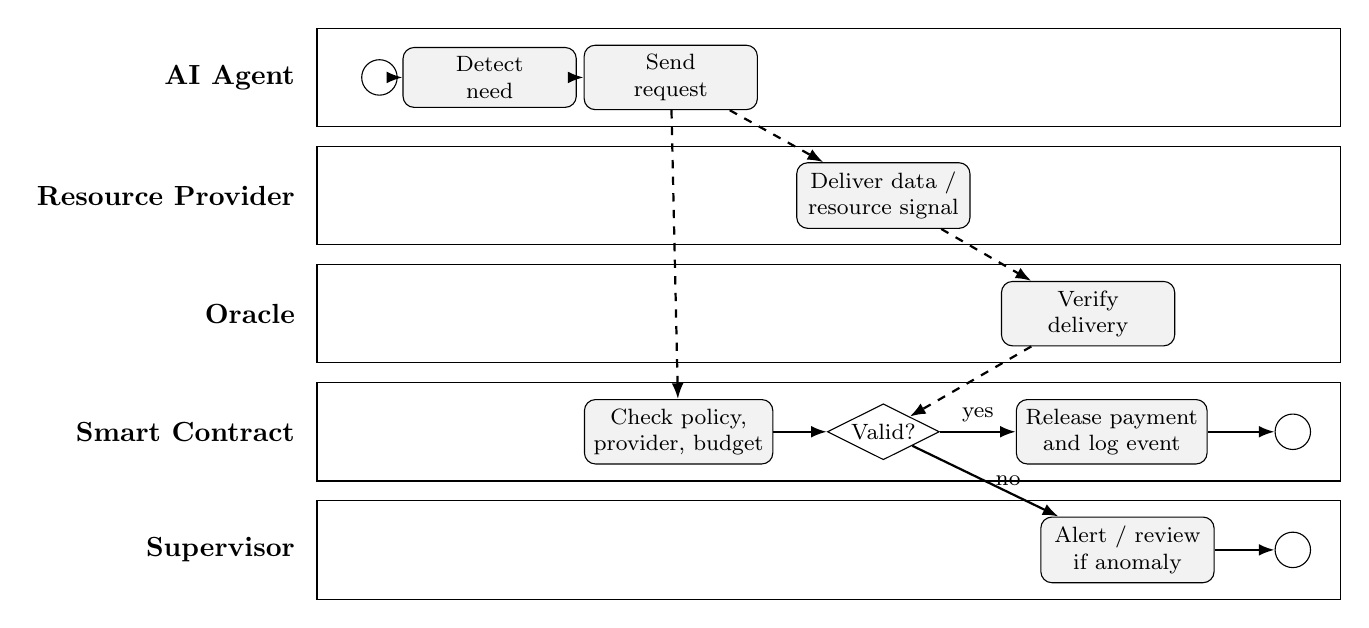
\begin{tikzpicture}[
    font=\footnotesize,
    lane/.style={draw, minimum width=13.0cm, minimum height=1.25cm, anchor=west},
    task/.style={draw, rounded corners, minimum width=2.2cm, minimum height=0.65cm, align=center, fill=gray!10},
    event/.style={draw, circle, minimum size=0.45cm, inner sep=0pt},
    gateway/.style={draw, diamond, aspect=2, align=center, inner sep=1pt},
    arr/.style={-{Latex[length=2mm]}, thick},
    msg/.style={dashed,-{Latex[length=2mm]}, thick}
]

\node[lane] (l1) at (0,0) {};
\node[lane] (l2) at (0,-1.5) {};
\node[lane] (l3) at (0,-3.0) {};
\node[lane] (l4) at (0,-4.5) {};
\node[lane] (l5) at (0,-6.0) {};

\node[anchor=east, font=\bfseries] at (-0.15,0) {AI Agent};
\node[anchor=east, font=\bfseries] at (-0.15,-1.5) {Resource Provider};
\node[anchor=east, font=\bfseries] at (-0.15,-3.0) {Oracle};
\node[anchor=east, font=\bfseries] at (-0.15,-4.5) {Smart Contract};
\node[anchor=east, font=\bfseries] at (-0.15,-6.0) {Supervisor};

\node[event] (start) at (0.8,0) {};
\node[task] (a1) at (2.2,0) {Detect\\need};
\node[task] (a2) at (4.5,0) {Send\\request};

\node[task] (p1) at (7.2,-1.5) {Deliver data /\\resource signal};

\node[task] (o1) at (9.8,-3.0) {Verify\\delivery};

\node[task] (s1) at (4.6,-4.5) {Check policy,\\provider, budget};
\node[gateway] (g1) at (7.2,-4.5) {Valid?};
\node[task] (s2) at (10.1,-4.5) {Release payment\\and log event};

\node[task] (h1) at (10.3,-6.0) {Alert / review\\if anomaly};
\node[event] (end) at (12.4,-4.5) {};
\node[event] (endno) at (12.4,-6.0) {};

\draw[arr] (start) -- (a1);
\draw[arr] (a1) -- (a2);
\draw[msg] (a2) -- (p1);
\draw[msg] (a2) -- (s1);
\draw[msg] (p1) -- (o1);
\draw[arr] (s1) -- (g1);
\draw[msg] (o1) -- (g1);
\draw[arr] (g1) -- node[above] {yes} (s2);
\draw[arr] (s2) -- (end);
\draw[arr] (g1) -- node[right] {no} (h1);
\draw[arr] (h1) -- (endno);

\end{tikzpicture}
\caption{BPMN-oriented process view of AI-agent micropayment execution}
\label{fig:bpmn_process}
\end{figure}

The process model follows core BPMN logic while remaining sufficiently compact for a report-oriented prototype. Both successful and rejected transaction paths terminate explicitly, improving clarity of exception handling and governance escalation.

Within the proposed architecture, the primary value object is a stable digital asset used for settlement. The smart contract acts as the main contract object implementing conditional execution logic. The most important data objects include service confirmations, transaction logs, proof references, and policy parameters. In practical deployments, most operational service data should remain off-chain. Only payment-relevant states and verification references should be anchored to the blockchain for auditability and execution control \citep{krueger2026workshop2,krueger2026workshop7a}.

\subsection{Blockchain Type, Consensus, and Architectural Choice}

The choice of blockchain type and consensus mechanism should follow practical requirements. For this use case, a public or hybrid smart-contract environment with low transaction costs appears more suitable than either a purely private chain or an expensive proof-of-work settlement layer. The main requirement is efficient programmable settlement for frequent low-value transactions.

Proof-of-stake environments and scalable smart-contract platforms therefore appear more plausible than proof-of-work systems for AI-agent micropayment scenarios \citep{krueger2026intro2,buterin2014ethereum}. This logic is also consistent with recent research on multi-agent economies integrating x402 micropayments and blockchain-based agent identities, where low-cost programmable settlement and public discoverability are treated as prerequisites for scalable autonomous agent ecosystems \citep{vaziry2025multiagent}.

A plausible baseline architecture would therefore involve a public permissionless or hybrid smart-contract platform with proof-of-stake consensus and relatively low transaction fees, potentially supported by Layer 2 infrastructure. Several operational arguments support this choice:

\begin{itemize}[leftmargin=1.2cm]
\item low transaction costs are necessary for micro-settlement;
\item programmable logic is required for conditional execution;
\item shared transaction state is needed across organizational boundaries;
\item public or hybrid environments improve interoperability;
\item scalable infrastructure improves the economics of high-frequency low-value transactions.
\end{itemize}

Therefore, a scalable proof-of-stake smart-contract environment appears more suitable than high-cost proof-of-work settlement architectures for this use case.

\subsection{Oracle Choice and Security}

Delegating payment authority to software is defensible only when that authority remains constrained. Smart accounts or similar programmable account structures can enforce spending limits, provider whitelists, category restrictions, and session-based permissions. A practical governance structure should distinguish between routine micro-transactions, medium-risk transactions requiring additional verification, and higher-risk operations requiring explicit human approval. This layered approach fits both operational logic and accountability requirements more effectively than unrestricted autonomous payment execution \citep{krueger2026workshop7b,europeanunion2024aiact}.

Oracle mechanisms remain central because the use case depends on verification of off-chain delivery conditions.   For real-time data purchases, software oracles provide the most natural baseline because the purchased resources are primarily digital. In DePIN-related scenarios or physical-resource access, hardware-based or reverse-oracle patterns become more relevant. In higher-value contexts, consensus-based oracle structures may reduce dependence on single external information sources and improve resilience against manipulation \citep{krueger2026oracles}.

\section{Prototype Elements}

This section adds three prototype-oriented elements to the proposed architecture: a process representation, a minimal smart contract, and a supervisory interface. The objective is not to deliver production-ready software, but to demonstrate how the business and governance logic described earlier can be translated into a technically plausible system design.

\subsection{Smart Contract Rules Before Code}

Before presenting code, the rules should be explicit. The selected use case can be translated into these core rules:

\begin{itemize}[leftmargin=1.2cm]
\item \textbf{If} the AI Agent requests a resource, \textbf{then} the smart contract checks whether the provider is approved, the amount is within policy limits, and enough balance exists.
\item \textbf{If} the provider delivers the requested service, \textbf{then} the oracle confirms the external condition.
\item \textbf{If} oracle confirmation exists and the request is valid, \textbf{then} payment is released to the provider.
\item \textbf{If} anomalies occur or policies are violated, \textbf{then} execution is paused or escalated to the human supervisor.
\end{itemize}

The logic is intentionally simple because the purpose of the prototype is to demonstrate the relationship between governance rules, verification logic, and programmable settlement rather than production-level optimization.


\subsection{Smart Contract Prototype}

A minimal Solidity prototype was prepared to illustrate how the operational logic can be implemented on-chain. The contract focuses on five mechanisms: approved providers, spending limits, oracle-based confirmation, supervisory pause control, and withdrawal of unused funds.

The architecture is deliberately constrained. A supervisor deposits funds, approves providers, assigns an oracle, and defines a maximum transaction amount. The AI Agent can create requests only for approved providers and only within predefined limits. Payment is released exclusively after oracle confirmation. The supervisor can also pause execution if abnormal behavior or operational risk is detected.

\begin{lstlisting}[style=solidity,caption={Minimal Solidity prototype for AI-agent micropayments},label={lst:solidity}]
pragma solidity ^0.8.20;

contract AIAgentMicropayment {
    address public owner;
    address public oracle;
    bool public paused;
    uint256 public maxAmountWei;

    struct Request {
        address requester;
        address provider;
        uint256 amount;
        string resourceId;
        bool fulfilled;
        bool paid;
    }

    uint256 public requestCount;
    mapping(uint256 => Request) public requests;
    mapping(address => bool) public approvedProviders;

    event ProviderApproved(address provider, bool approved);
    event OracleUpdated(address oracle);
    event MaxAmountUpdated(uint256 maxAmountWei);
    event FundsDeposited(address from, uint256 amount);
    event FundsWithdrawn(address to, uint256 amount);
    event RequestCreated(
        uint256 indexed requestId,
        address indexed requester,
        address indexed provider,
        uint256 amount,
        string resourceId
    );
    event DeliveryConfirmed(uint256 indexed requestId);
    event PaymentReleased(uint256 indexed requestId, address indexed provider, uint256 amount);
    event Paused(bool status);

    modifier onlyOwner() {
        require(msg.sender == owner, "Not owner");
        _;
    }

    modifier onlyOracle() {
        require(msg.sender == oracle, "Not oracle");
        _;
    }

    modifier notPaused() {
        require(!paused, "Contract paused");
        _;
    }

    constructor(address _oracle, uint256 _maxAmountWei) {
        require(_oracle != address(0), "Oracle required");
        owner = msg.sender;
        oracle = _oracle;
        maxAmountWei = _maxAmountWei;
    }

    receive() external payable {
        emit FundsDeposited(msg.sender, msg.value);
    }

    function deposit() external payable onlyOwner {
        emit FundsDeposited(msg.sender, msg.value);
    }

    function withdraw(uint256 amount) external onlyOwner {
        require(address(this).balance >= amount, "Insufficient balance");
        payable(owner).transfer(amount);
        emit FundsWithdrawn(owner, amount);
    }

    function setOracle(address _oracle) external onlyOwner {
        require(_oracle != address(0), "Invalid oracle");
        oracle = _oracle;
        emit OracleUpdated(_oracle);
    }

    function setMaxAmount(uint256 _maxAmountWei) external onlyOwner {
        require(_maxAmountWei > 0, "Limit required");
        maxAmountWei = _maxAmountWei;
        emit MaxAmountUpdated(_maxAmountWei);
    }

    function approveProvider(address provider, bool approved) external onlyOwner {
        require(provider != address(0), "Invalid provider");
        approvedProviders[provider] = approved;
        emit ProviderApproved(provider, approved);
    }

    function setPaused(bool _paused) external onlyOwner {
        paused = _paused;
        emit Paused(_paused);
    }

    function requestResource(
        address provider,
        uint256 amount,
        string calldata resourceId
    ) external notPaused returns (uint256) {
        require(approvedProviders[provider], "Provider not approved");
        require(amount > 0, "Amount must be > 0");
        require(amount <= maxAmountWei, "Amount exceeds limit");
        require(address(this).balance >= amount, "Insufficient contract balance");

        requestCount += 1;
        requests[requestCount] = Request({
            requester: msg.sender,
            provider: provider,
            amount: amount,
            resourceId: resourceId,
            fulfilled: false,
            paid: false
        });

        emit RequestCreated(requestCount, msg.sender, provider, amount, resourceId);
        return requestCount;
    }

    function confirmDelivery(uint256 requestId) external onlyOracle notPaused {
        Request storage r = requests[requestId];
        require(r.amount > 0, "Invalid request");
        require(!r.fulfilled, "Already fulfilled");

        r.fulfilled = true;
        emit DeliveryConfirmed(requestId);
    }

    function releasePayment(uint256 requestId) external notPaused {
        Request storage r = requests[requestId];
        require(r.amount > 0, "Invalid request");
        require(r.fulfilled, "Delivery not confirmed");
        require(!r.paid, "Already paid");
        require(approvedProviders[r.provider], "Provider no longer approved");
        require(address(this).balance >= r.amount, "Insufficient balance");

        r.paid = true;
        payable(r.provider).transfer(r.amount);

        emit PaymentReleased(requestId, r.provider, r.amount);
    }
}
\end{lstlisting}

The contract design implements an escrow mechanism, requiring the Human Supervisor to pre-fund the architecture via the \texttt{deposit} function before the AI Agent can successfully invoke \texttt{requestResource}.

The prototype intentionally omits production-level mechanisms such as multi-signature approval, tokenized settlement assets, provider staking, dispute resolution, oracle consensus, rate limiting, and advanced security controls. Nevertheless, it demonstrates the central architectural principle of the report: payment authority can be delegated to software only when execution remains bounded by explicit governance rules and verifiable delivery conditions.

\subsection{Supervisor Dashboard Mock-up}

Although the proposed architecture is primarily machine-to-machine, human supervision remains necessary. The purpose of the supervisory interface is not manual execution of payments, but definition of operating boundaries, provider approval, monitoring of activity, and intervention in anomalous situations. The interface therefore reflects controlled and auditable automation rather than unrestricted autonomous financial behavior.

\begin{figure}[H]
\centering
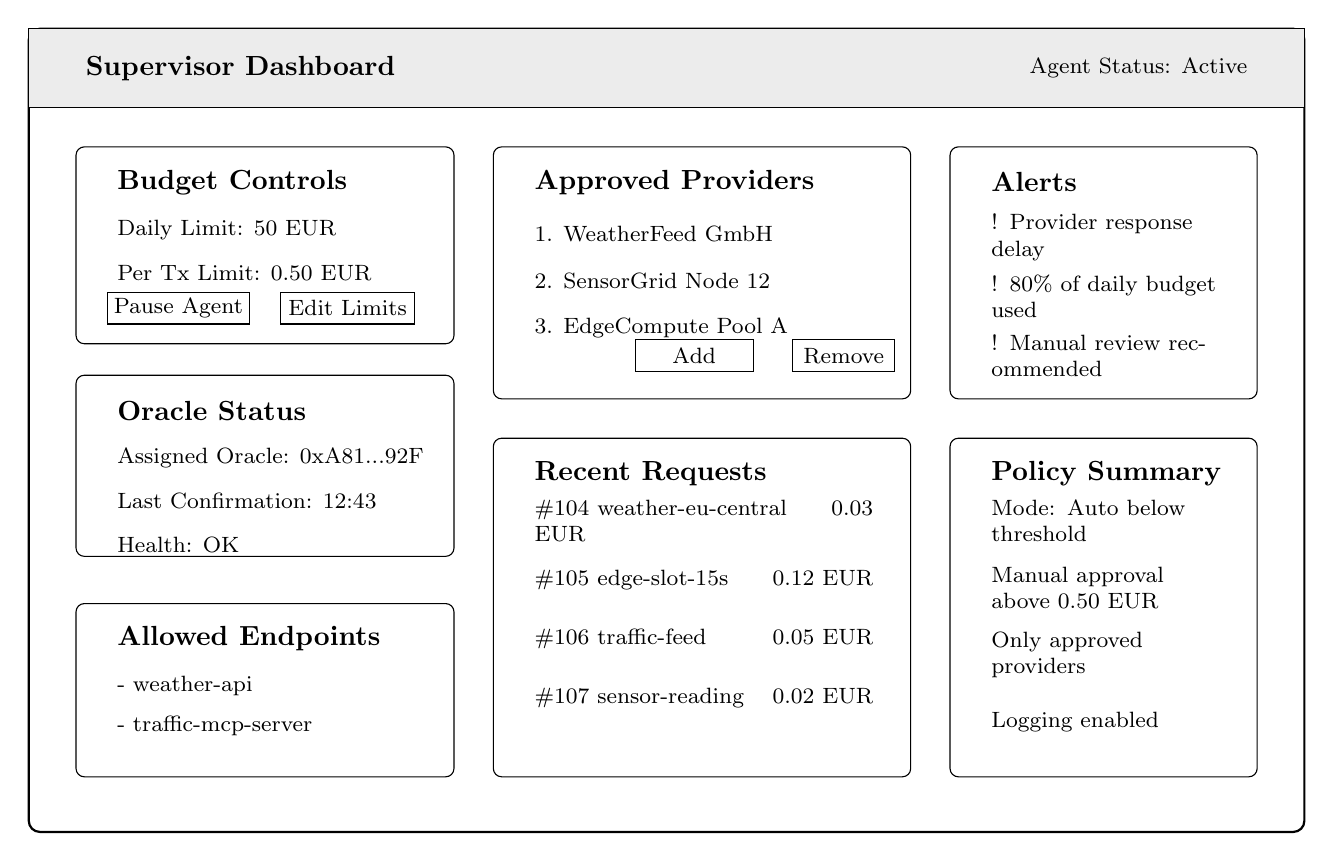
\begin{tikzpicture}[font=\footnotesize]

\draw[rounded corners=4pt, thick] (0,0) rectangle (16.2,10.2);

\draw[fill=gray!15] (0,9.2) rectangle (16.2,10.2);
\node[anchor=west, font=\bfseries] at (0.6,9.7) {Supervisor Dashboard};
\node[anchor=east] at (15.6,9.7) {Agent Status: Active};

\draw[rounded corners=3pt] (0.6,6.2) rectangle (5.4,8.7);
\node[anchor=west, font=\bfseries] at (1.0,8.25) {Budget Controls};
\node[anchor=west] at (1.0,7.65) {Daily Limit: 50 EUR};
\node[anchor=west] at (1.0,7.10) {Per Tx Limit: 0.50 EUR};

\draw (1.0,6.45) rectangle (2.8,6.85);
\node at (1.9,6.65) {Pause Agent};
\draw (3.2,6.45) rectangle (4.9,6.85);
\node at (4.05,6.65) {Edit Limits};

\draw[rounded corners=3pt] (0.6,3.5) rectangle (5.4,5.8);
\node[anchor=west, font=\bfseries] at (1.0,5.35) {Oracle Status};
\node[anchor=west] at (1.0,4.75) {Assigned Oracle: 0xA81...92F};
\node[anchor=west] at (1.0,4.20) {Last Confirmation: 12:43};
\node[anchor=west] at (1.0,3.65) {Health: OK};

\draw[rounded corners=3pt] (0.6,0.7) rectangle (5.4,2.9);
\node[anchor=west, font=\bfseries] at (1.0,2.45) {Allowed Endpoints};
\node[anchor=west] at (1.0,1.85) {- weather-api};
\node[anchor=west] at (1.0,1.35) {- traffic-mcp-server};

\draw[rounded corners=3pt] (5.9,5.5) rectangle (11.2,8.7);
\node[anchor=west, font=\bfseries] at (6.3,8.25) {Approved Providers};
\node[anchor=west] at (6.3,7.60) {1. WeatherFeed GmbH};
\node[anchor=west] at (6.3,7.00) {2. SensorGrid Node 12};
\node[anchor=west] at (6.3,6.40) {3. EdgeCompute Pool A};

\draw (7.7,5.85) rectangle (9.2,6.25);
\node at (8.45,6.05) {Add};
\draw (9.7,5.85) rectangle (11.0,6.25);
\node at (10.35,6.05) {Remove};

\draw[rounded corners=3pt] (5.9,0.7) rectangle (11.2,5.0);
\node[anchor=west, font=\bfseries] at (6.3,4.55) {Recent Requests};

\node[anchor=west, align=left, text width=4.3cm] at (6.3,3.95)
{\#104 weather-eu-central \hfill 0.03 EUR};

\node[anchor=west, align=left, text width=4.3cm] at (6.3,3.20)
{\#105 edge-slot-15s \hfill 0.12 EUR};

\node[anchor=west, align=left, text width=4.3cm] at (6.3,2.45)
{\#106 traffic-feed \hfill 0.05 EUR};

\node[anchor=west, align=left, text width=4.3cm] at (6.3,1.70)
{\#107 sensor-reading \hfill 0.02 EUR};

\draw[rounded corners=3pt] (11.7,5.5) rectangle (15.6,8.7);
\node[anchor=west, font=\bfseries] at (12.1,8.25) {Alerts};

\node[anchor=west, align=left, text width=3.0cm] at (12.1,7.55)
{! Provider response delay};

\node[anchor=west, align=left, text width=3.0cm] at (12.1,6.80)
{! 80\% of daily budget used};

\node[anchor=west, align=left, text width=3.0cm] at (12.1,6.05)
{! Manual review recommended};

\draw[rounded corners=3pt] (11.7,0.7) rectangle (15.6,5.0);
\node[anchor=west, font=\bfseries] at (12.1,4.55) {Policy Summary};

\node[anchor=west, align=left, text width=3.0cm] at (12.1,3.95)
{Mode: Auto below threshold};

\node[anchor=west, align=left, text width=3.0cm] at (12.1,3.10)
{Manual approval above 0.50 EUR};

\node[anchor=west, align=left, text width=3.0cm] at (12.1,2.25)
{Only approved providers};

\node[anchor=west, align=left, text width=3.0cm] at (12.1,1.40)
{Logging enabled};

\end{tikzpicture}
\caption{Wireframe of a human supervisory dashboard for bounded AI-agent payments}
\label{fig:dashboard_mock}
\end{figure}

The dashboard supports governance rather than direct operational execution. A supervisor can define spending limits, approve providers, monitor transaction activity, observe oracle health, and intervene when anomalies appear. This preserves human accountability while still allowing high-frequency automated settlement within predefined boundaries.

\section{Regulatory Context, Critical Discussion, and Conclusion}

The proposed model operates at the intersection of digital assets and autonomous decision-making. On the financial side, MiCA defines the European regulatory framework for crypto-asset services and stablecoin-related infrastructure \citep{europeanparliament2023mica}. On the AI side, the AI Act emphasizes accountability, transparency, and human responsibility in systems with financial or operational consequences \citep{europeanunion2024aiact}. For this reason, the proposed architecture combines automation with human supervision instead of allowing unrestricted financial autonomy for software agents.

The main argument for the proposed architecture is that it addresses a practical mismatch between AI-driven micro-consumption and traditional payment infrastructure. The model supports small, programmable, and auditable transactions in a multi-party environment. At the same time, some parts of this functionality are already emerging in commercial solutions. Stripe supports usage-based and automated billing for digital services and introduced the Machine Payments Protocol (MPP) for programmatic agent payments. Coinbase introduced x402 as an HTTP-native payment protocol for automatic stablecoin settlement and also developed agent-oriented wallet infrastructure with policy controls. Crossmint provides wallets, stablecoin balances, spending limits, whitelisting, audit logs, and human approval workflows for agentic payments. Nevermined focuses directly on delegated spending and real-time settlement for AI-native services. However, these solutions still depend largely on centralized platforms, trusted intermediaries, or predefined payment rails.

The limitations of blockchain should also be stated clearly. Blockchain is not automatically the best solution for every payment or automation problem. If transaction values are large, actors already trust each other, or centralized systems operate efficiently, conventional infrastructure may remain simpler and cheaper. Blockchain also does not eliminate the oracle problem. Weak or unreliable external verification still produces weak system outputs, even when settlement itself is automated. The proposed architecture should therefore be understood as a focused solution for situations where micropayment granularity, conditional execution, cross-organizational interoperability, and programmable settlement are all required simultaneously \citep{krueger2026oracles,defilippi2018law}.

The prototype elements increase the practical credibility of the concept. The BPMN-oriented process model clarifies the operational workflow. The Solidity prototype demonstrates that the business logic can be translated into explicit programmable rules. The dashboard mock-up shows how human supervision can remain part of the system through policy controls, monitoring, and escalation mechanisms. Together, these elements move the report beyond abstract discussion toward a technically plausible architecture.

The conclusion of the report is intentionally limited. AI Agents do not require crypto-payment in every scenario. However, in selected machine-to-machine contexts involving high-frequency, low-value, condition-based transactions, blockchain-based payment infrastructure provides meaningful advantages over conventional systems. The strongest use case identified in this report is the autonomous purchase of real-time data and narrowly scoped digital resource units. In this context, blockchain creates value not because it is novel, but because it supports transaction patterns that traditional payment systems handle inefficiently.
\newpage
\bibliographystyle{apalike}
\bibliography{bibliography}
\addcontentsline{toc}{section}{References}

\end{document}
